\chapter{Design}
\label{chap:design}
\lhead{\emph{Design}}


This chapter will address the design features and prototypes tested and surveyed on the applicants. An excessive amount of research has been carried out in the area of applying AR in a school environment, the existing research available is on non-autistic Children and a physical book, an example of marker AR, is needed for the functionality to work. This research paper will examine the use of AR for the education of Children with ASD and the benefits and effectiveness of modern day AI for Children with learning disabilities and who are on the Autism spectrum. 


\subsection{Requirements} 

There has been a rise in the use of touch screen assistive technology as a tool for intervention and interdisciplinary research for children with autism. This area can be challenging as the process for designing for a group of individuals who have a profile that is unique to them and experience the world differently to a typical person will be challenging [X]. https://www.sciencedirect.com/science/article/pii/S1877042816000471

An important aspect when designing an assistive tool for children with autism is the user interface (UI), the interface or the face of the technology plays a vital part for an applications success. The user interface when designed and developed for the target market can make the experience enjoyable, easy to use and the user will return, alternatively if the user interface has not been designed or developed to the requirements of the targeted user then they will have a poor experience and it will be of no or little benefit to the user. There has been research carried out in the in the accessibility in regards to people with visual, hearing and physical impairments, there disabilities differ vastly to people with autism who have specific repetitive behaviours and patterns.

When designing an interface for individuals, when possible an accessibility specialist should be present on the design team to give recommendations. When this is not possible, the design should influenced by the users and educational professionals who will be using the application with the children who are autistic and will also need an understanding of how the application works and the benefit of the technology [X]. The UK Department of Health created a methodology for the preparation of documents for people with learning disabilities [X], the 14 rules are:

\begin{table} [h]
    \centering
\begin{tabular}{ | m{2em} | m{7cm}|} 
\hline
1 & Each idea needs both words and pictures.   \\ 
\hline
2 & Pictures and words go next to each other, this helps more people to understand the information. \\ 
\hline
3 & Make sure that it is clear which pictures support which part of the text. \\ 
\hline
4 & Pictures must be easy to understand. \\ 
\hline
5 & Pictures should go on the left. \\ 
\hline
6 & Pictures can be drawings, photographs or images. \\
\hline
7 & Make sure that pictures are as big as possible.  \\
\hline
8 & Words must be easy to understand. \\
\hline
9 & If you use difficult words, say what they mean using easy words. \\
\hline
10 & Words go on the right. \\
\hline
11 & Words must be written clearly, a font like Arial is good. \\
\hline
12 & Words must be big in size, a font size of at least 14 point is good. \\
\hline
13 & Sentences must be sort, no more than 15 words. \\
\hline
14 & Documents to be no more than 20 pages. \\
\hline
\end{tabular}
\centering
\caption{Table of rules for designing for disabilities}
    \label{tab:my_label}
\end{table}

The rules created for the preparation of documents for people with learning disabilities are very basic. They have tried to simplify the rules for designers in regards to documents, the research did not specify if these rules could be used for both digital and physical documents. The rules do not incorporate or refer to colours used when creating a document for people with learning disabilities. 
\newpage
Another methodology that has been created by Freyhoff, Hess, Kerr, Tronbacke and Van Der Veken in their “Make it Simple: European Guidelines for the Production of Easy to Read Information for People with Learning Disability for authors, editors, information providers, translators and other interested persons” [X]. This report forms part of a project to develop “Easy to Read Guide-lines” for EU languages to ensure easy access to information for people with a language disability. The additional recommendation on design on the layout include:

\begin{itemize}
    \item Do not use an image as the background of text.
    \item Try to have one sentence on one line.
    \item Try to minimise information.
    \item Use a maximum of two typefaces per layout.
    \item Do not use block capitals, use underlining or bold to emphasis a word.
    \item Use headings as navigational aids.
    \item Use the full date format, for example Saturday, 26 September 2021.
    \item Phone numbers should be separated, for example 123 456 789.
    \item Numerals should be used rather than the word equivalent, for example 10 should be used instead of the word equivalent ten.
    \item Roman numerals should never be used.
\end{itemize}

These additional recommendations give a better insight into what the requirements are when designing with text for documents and applications for people with a learning and language disability.

\subsection {Multimedia Requirement}

The user interface experience is critical to the applications success as discussed. A lack design elements created to target the users who are autistic can result in a poor experience, similarly if the application is too media rich, over stimulating the users senses and causing a poor experience as well. When it comes to the multimedia requirements it can be noted that personalising is a key element for an applications success. This ensures a person with ASD has their needs met. 

\subsection{Design} 


Following research on Augmented Reality, task-oriented instructions and design principles, this section proposes how task instructions will be delivered in a prototype. The prototype is designed to simulate how task instructions may be delivered in a real Augmented Reality environment. Human-computer interaction

Human-computer interaction (HCI) has developed extensively in recent years; there has been an interest in implementing HCI into education~\cite{Reference24}. in Comparison with traditional approaches in the real world, AR gesture and AI voice recognition are  an alternative since they are interactive and can be customised based on the user.  This article implemented a prototype based on an augmented reality system and the principles and fundamentals of interactive design. Accessibility to the Children is achieved by handheld devices and the dynamic switch of AR gesture and AI voice recognition. By this interactive method, children can interact with the virtual objects easily and naturally and at their own pace and level. 

An example of AR gesture technology through gamification is the Xbox Kinect; the device's software makes the Kinect an excellent example of AR and AI recognition for gaming. Data is collected from the game regarding motion-capture of actually moving things in real-life environments. The Kinect processes the data using an artificial intelligence machine-learning algorithm allowing the Kinect to map the visual data it collects to models representing people of different backgrounds, such as age, height and environment of the user. This information is how the devices learn. The extracted information from the Kinect goes through a data processing system; it can be difficult to ensure the accuracy and efficiency of the information. To enhance the efficiency of the capture of gestures, a company in America produces a special motion controller called  Leap  Motion,  which can specifically recognise fingers and interact with gestures~\cite{Reference25}. Both static and dynamic information is taken to ensure high performing systems for the users, so the device feels natural, accurate and easy to use~\cite{Reference26}.

The Kinects design is high tech and contains three pieces that work together to detect the user's motion and creates a physical image on the screen. These three pieces are;
\begin{itemize}
    \item An RGB colour VGA video camera detects the user's facial features and body type.
    \item A depth sensor that uses a monochrome CMOS sensor and infrared projector that create 3D imagery; it also measures distance in the room by transmitting invisible near-infrared light and measures "time of flight" after reflecting off an object. 
    \item A multi-array microphone that can isolate voices of the players from the background noise, this AI features allows its users to use their voice as a control feature.
\end{itemize}

These combined components can detect and are able to track 48 different points on each of the player's bodies and repeat the process 30 times every second~\cite{Reference27}.


\begin{figure}[h]
\centering
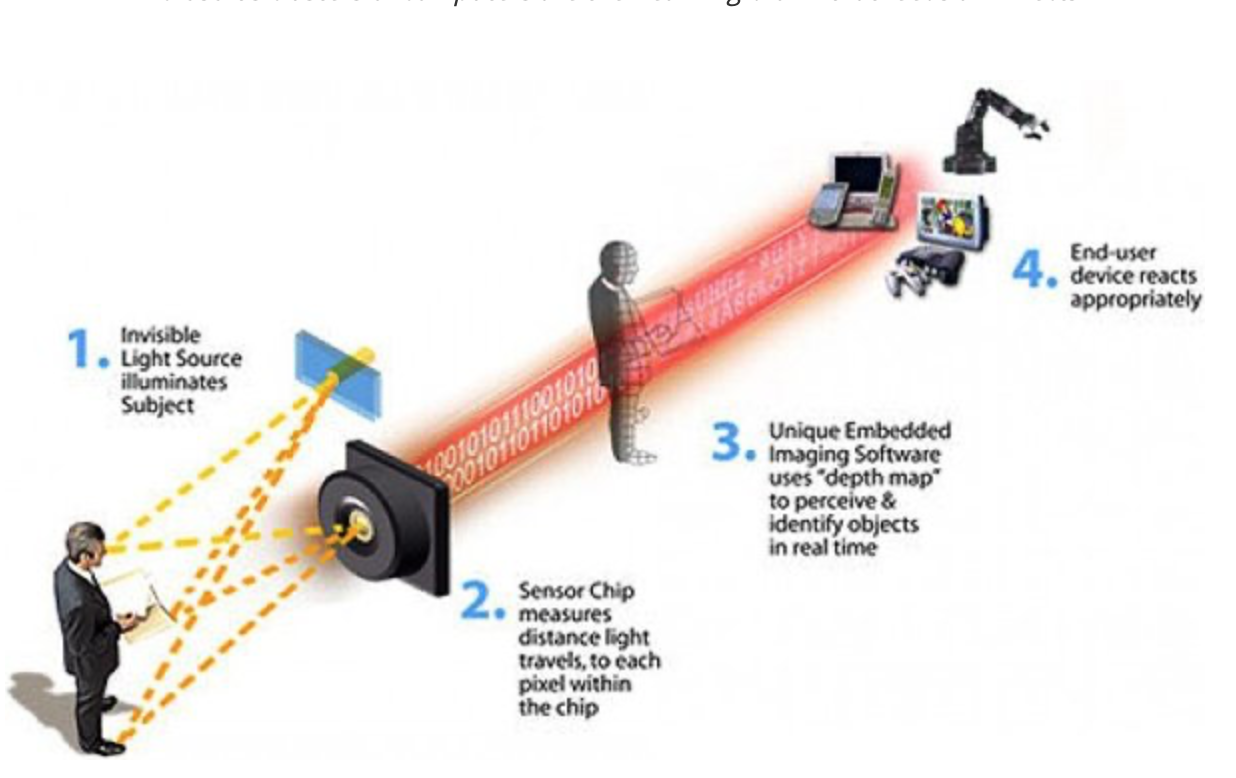
\includegraphics[width=1.0\textwidth]{IDD_LauraMartin_R00124705/Figures/infared.png}
\caption{Explanation of Infrared}
{here goes expl}
\end{figure}



\begin{figure}[h]
\centering
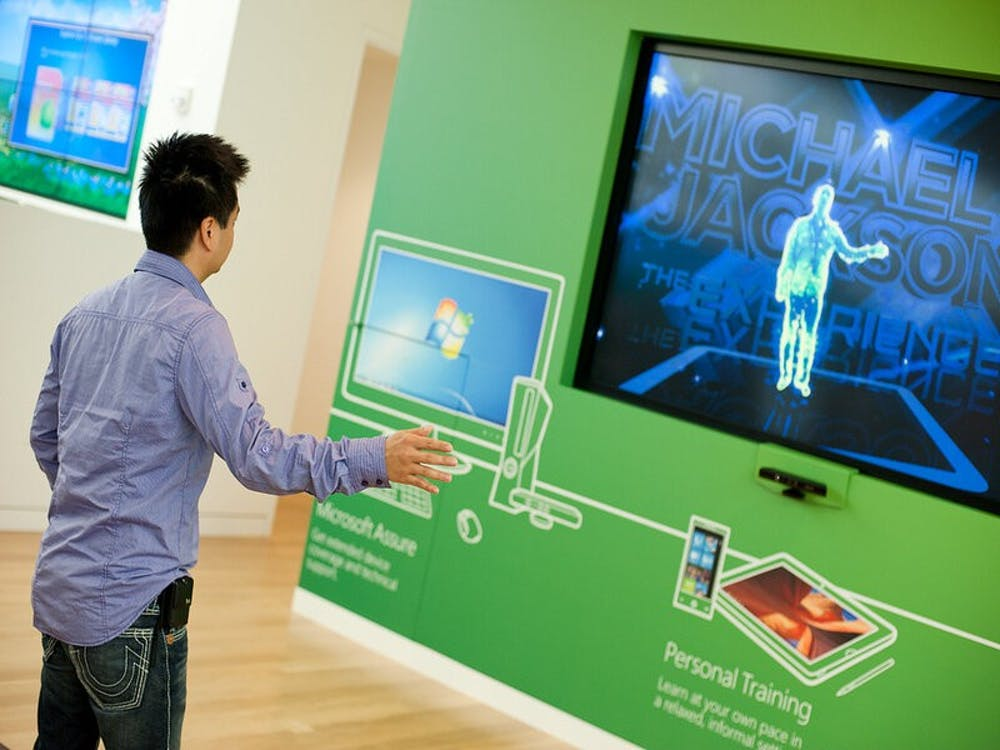
\includegraphics[width=0.5\textwidth]{IDD_LauraMartin_R00124705/Figures/kinect.jpg}
\caption{Kinect in use}
{here goes expl}
\end{figure}

The below images summerise the above images ccccc
figure 3.2 cccc
figure 

\subsection{Existing Design}
The problem with existing information and research that is available is that it requires a physical book or QR code, also known as marker AR to work and that is not always practical. The other problem is that the information in existence is to help a Child with ASD develop to function in a society for individuals who are non-Autistic or considered typical, existing applications teach a Child with ASD to be judged based on facial expressions, for example the paper spoken about earlier and the application Emotrain which is a facial expression recognition tool that judges a Child with ASD and their ability to show emotion and how to react in society and when communicating with other people. This can be challenging for an individual with ASD as they are considered to be literal thinkers and find it difficult to be imaginative with other individuals emotions and have difficulties in portraying their own emotions. The application Emotrain is too general and broad and is not individualised to each user who is Autistic, each person has a different set of characteristics and repetitive patterns, even though they may be similar, the patterns and behaviours will not present as the same and will have various triggers. 

Another area of concern from the application Emotrain is the development of ‘Affectiva’ used by the authors and developers of the Emotrain application, the Affectiva development was created for businesses to understand their customers and was also implemented in the Emotrain application. This is a concern because Affectiva was never developed with the Autistic demographic in mind and the process was never adapted or improved for the use of individuals with Autism, this is an issue due to the Affectiva functionality being too broad and general and not individualised [X]. The consequences of this problem if not resolved are the Autistic users using an application that is not targeted towards them and may have difficulty understanding the application. Another application targeted towards children with autism is 'TaLNA', this application is based on improving the users understanding of basic numeral literacy and calculations. This application claims to boost the child's engagement to learn, to memorise and to recognise numbers through the animated and interactive learning processes. The problem with this application is that it is very narrow and is only targeted to autistic individuals who have difficulty with numeracy comprehension. [X]


The solution this paper and prototype proposes is to develop a markerless AR application, designed through the analysis of existing information, surveys, interviews and prototype testing on applicants with Autism, a parent/guardian of the applicant and Autism educational professionals. It will be an application designed for individuals with Autism and learning disabilities to help them to progress with their academic studies through gamification, AR and AI functionalities. This proposed design will cover all aspects of the educational program taught.

\subsection{Problem Definition}
The problems seen in the market of applications aimed towards children with autism is the user interface is that there are limited guidelines for the user interface (UI) of an applications for children with autism. The design in existing applications is unexplored and unproven and can make the experience for the child with autism increasingly more difficult than it needs to be. A study has been conducted as to what are the main usability factors to consider when design a mobile applications for children with autism. The study researched 23 recent works that followed a set of 6 usability factors, those factors were;

\begin{itemize}
  \item Easy to use
  \item Effectiveness
  \item Understandable
  \item Satisfaction
  \item Appearance
  \item Efficiency
\end{itemize}

 \begin{figure}[h]
\centering
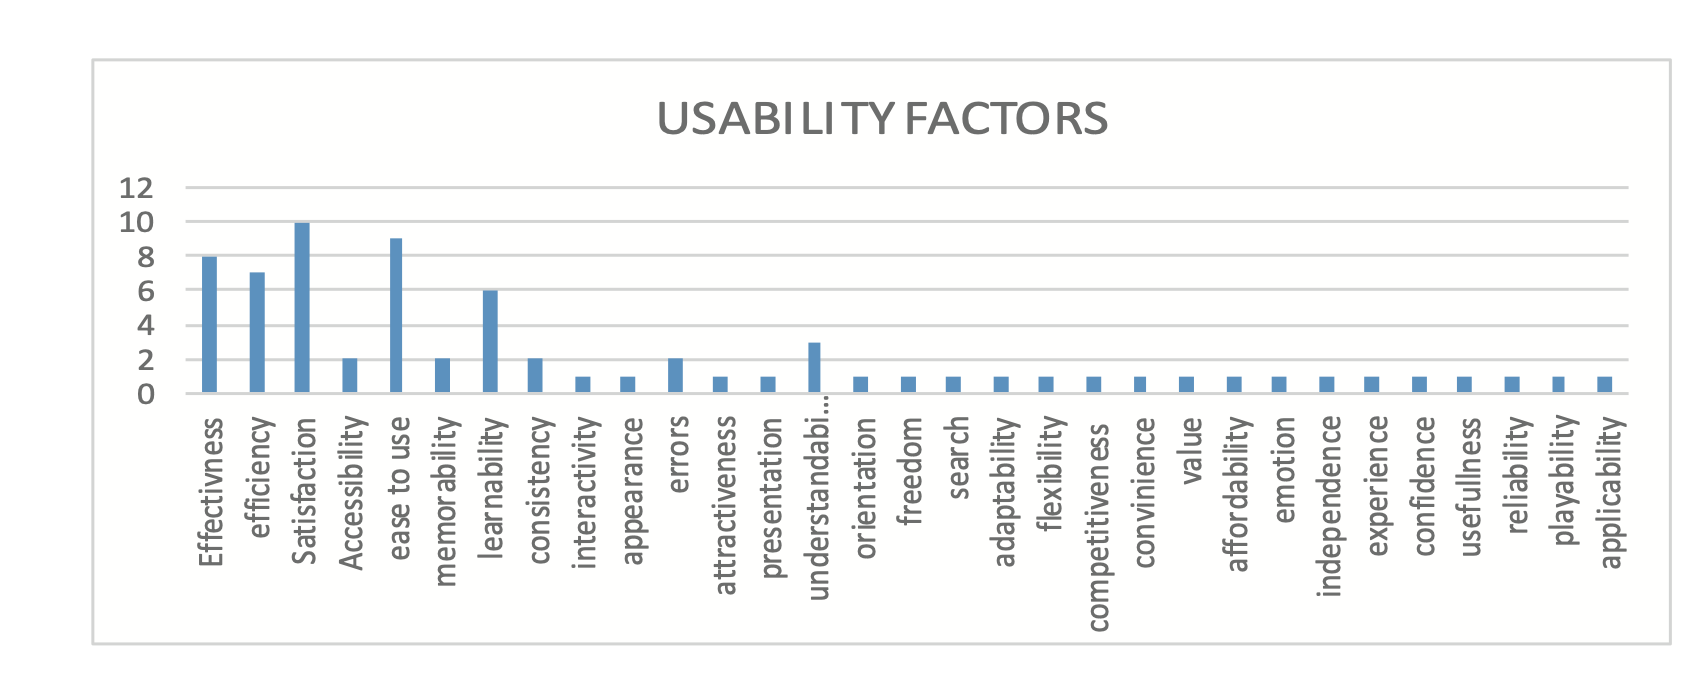
\includegraphics[width=1.0\textwidth]{IDD_LauraMartin_R00124705/Figures/usabilityfactors.png}
\caption{Usability factors}
\end{figure}

To summarise the above figure (figure 3.1), 31 design elements have been identified in the [X] research paper. These elements identify the requirements to be met when designing a mobile application to make it as effective and efficient as possible. 

The problem defined with existing applications outlined in section 3.0.3 is that the existing applications are either too broad, meaning it is not designed for children with autism, but is designed for those who have typical behaviours and patterns. The other problem is the applications being too narrow, meaning the application only covers one area of difficulty, more applications will be needed for the other problem areas, therefor different design and a non-consistent experience for the user.


\subsection{Augmented reality effectiveness in design}
This chapter should include the most relevant/important code listing and discuss relevant/interesting aspects; explain features you wish to highlight. 

\subsection{AI Effectiveness in design}


 

%Provide a high level view of the system and then break down the system. Include any packages or components you are using (the versions of these should be given) and what they are responsible for and what they communicate to. You need to be as specific here as you can. If you have a hardware element in your project this is also where you provide a high level view of how these elements integrate into the project. So for a project that is cyber-physical you will have both a hardware and software architecture diagram.


